% filepath: Figures/tikz2pdf/diagram/xFeat_ImageNet256_mAcc_standalone.tex
\documentclass[tikz,border=6pt]{standalone}
\usepackage{tikz}
\usepackage{pgfplots}
\pgfplotsset{compat=1.18} % passe ggf. an deine TeX-Installation an

% Falls das Hauptdokument Variablen/Makros wie \VarPicWidthD definiert,
% überschreibe sie nicht: providecommand verwendet nur einen Ersatz wenn nicht vorhanden.
\providecommand{\VarPicWidthD}{0.9\textwidth}

% Falls du in den tikz-Files \acs o.ä. verwendest: einfache Ersatzdefinitionen
\providecommand{\acs}[1]{#1}

\begin{document}
% Input des originalen TikZ-Codes (relativer Pfad zum Ordner dieses Files)
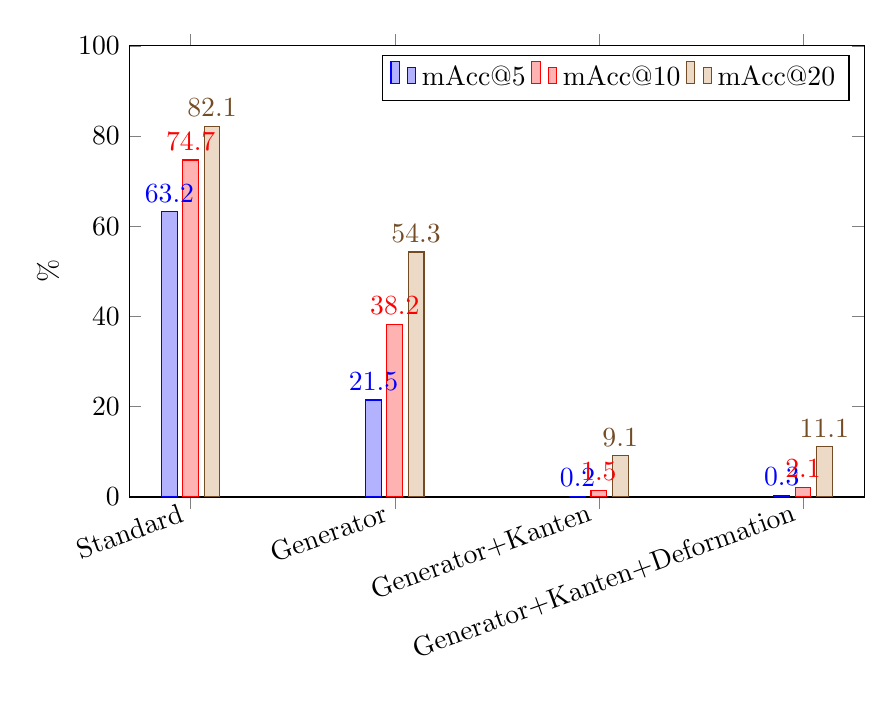
\begin{tikzpicture}
    \begin{axis}[
        ybar,
        bar width=0.2cm,
        width=\VarPicWidthD,
        height=0.67*\VarPicWidthD,
        ylabel={\%},
        symbolic x coords={Standard, Generator, Generator+Kanten, Generator+Kanten+Deformation},
        xtick=data,
        x tick label style={rotate=20, anchor=east}, % <--- hier Labels drehen
        legend style={at={(0.98,0.98)}, anchor=north east, legend columns=-1},
        nodes near coords,
        ymin=0, ymax=100
    ]
        \addplot coordinates {(Standard,63.2) (Generator,21.5) (Generator+Kanten,0.2) (Generator+Kanten+Deformation,0.3)};
        \addplot coordinates {(Standard,74.7) (Generator,38.2) (Generator+Kanten,1.5) (Generator+Kanten+Deformation,2.1)};
        \addplot coordinates {(Standard,82.1) (Generator,54.3) (Generator+Kanten,9.1) (Generator+Kanten+Deformation,11.1)};
        \legend{mAcc@5,mAcc@10,mAcc@20}
    \end{axis}
\end{tikzpicture}

\end{document}